\section{Dark energy, distances, and the primary CMB fit}
\label{sec:cosmology}

The geodesic-clock release model gives fits close to \LCDM\ on Planck
primary CMB spectra, DESI DR2 baryon acoustic oscillations, and
DES-Dovekie supernova distances. The standard linear-depletion
configuration uses $\sum m_\nu=0.06\,$eV, the Dovekie likelihood as
released, nonlinear lensing from each model's perturbations, and a free
Planck calibration with prior $1\pm0.0025$. It gives
$\Delta\chi^2=+0.85$, with five cosmological parameters for release and
six for \LCDM. The configuration with massless neutrinos, fixed
calibration, nonlinear lensing and a free supernova offset below $z=0.1$
gives $\Delta\chi^2=-0.39$. \source{C6}

The exponential positive-allocation fit uses massless neutrinos, fixed
calibration, linear lensing and the low-redshift offset. It gives
$\Delta\chi^2=-0.5152$; a separate archived linear-depletion fit with
the same likelihood settings gives $-0.5186$. Their relative scores differ
by about $0.0034$, with different numerical accuracy settings contributing
to the comparison. Their \LCDM\ reference is $2228.316$, against
$2228.359$ for the one-harness comparison of Section~\ref{sec:distances}.
Its conversion fraction is
$\eta_*=0.0298668$, its initial commitment abundance is tied to baryons,
and one parameter sets the mixing time. \source{C4, C5}

The hydrodynamic calculation tests the release normalization. With the
retention gate taken from the halo occupation of feedback-resolved
simulations and no input adjusted to the vacuum density, it gives
$\Omega_\Lambda=0.709\pm0.02$ against the likelihood value $0.707$. With the
reionization redshift taken from the fitted optical depth, that frozen
history fits the CMB, BAO and supernova data with four cosmological
parameters at $\Delta\chi^2=+1.07$ against six-parameter \LCDM
(Section~\ref{sec:coolinggate}).

\subsection{What the expansion measurements constrain}

In a homogeneous universe, the scale factor $a(t)$ measures relative
expansion and $H=\dot a/a$. Nonrelativistic matter of conserved comoving
mass has density proportional to $a^{-3}$. A vacuum component with
pressure $p_\Lambda=-\rho_\Lambda$ has constant density when it exchanges
no energy with other components. Throughout this section, energy-density
equations use $c=1$.

The observations constrain this expansion through complementary physical
scales. Supernovae supply relative luminosity distances,
\begin{equation}
D_L(z)=(1+z)c\int_0^z\frac{dz'}{H(z')}
\end{equation}
in a spatially flat universe. Their absolute magnitude and calibration
must be inferred along with the cosmology. Baryon acoustic oscillations
compare the transverse distance $D_M$ and radial distance $D_H=c/H$ with
the sound horizon $r_d$. The CMB fixes the early baryon and gravitating
matter densities, the primordial fluctuation spectrum, and the angular
size of the acoustic scale. A competitive joint fit must reproduce the
early acoustic physics as well as the late distance relation.
\cite{desi,planck}

In the capacity model, committed material exists before the acoustic
epochs and acts approximately as collisionless matter. Subsequent
structure formation transfers part of its energy into the vacuum sector.
This timing allows an early gravitating component and a late accelerating
component to share an origin. The theory specifies an effective formation map and
pre-acoustic epoch in O.15. Its microscopic formation vertex remains open;
the abundance and subsequent release retain the stated ledger assumptions.

\subsection{The record that mixing can destroy}

An assembled baryonic object has a collective source identity: its
constituents can be associated with a particular progenitor. Let $A$
denote that progenitor label and $Y_t$ a physically specified resolution
of the baryonic state at time $t$. The mutual information
\begin{equation}
I(A;Y_t)=\sum_{A,Y}p(A,Y;t)
\ln\frac{p(A,Y;t)}{p(A)p(Y;t)}
\end{equation}
measures how much the resolved state tells us about the progenitor.
For a fixed cohort and label alphabet, the normalized identity loss is
\begin{equation}
K_{\rm mix}(t)=1-\frac{I(A;Y_t)}{H(A)}
=\frac{H(A\mid Y_t)}{H(A)}.
\label{eq:informationkernel}
\end{equation}
It is zero when the progenitor can be recovered perfectly and approaches
one when the resolved state carries no information about that label.

Irreversible mixing gives this definition a dynamical basis. Suppose the
mass fraction $c_A(\boldsymbol x,t)$ of each label is advected by the same
velocity field and diffuses with the same positive semidefinite tensor
$D$. For a closed cohort of gas mass $M_g$, fixed label fractions, and
vanishing boundary flux, the resolved continuum information obeys
\begin{equation}
\frac{dI}{dt}=-\frac{1}{M_g}\sum_A
\int \frac{\rho}{c_A}
(\boldsymbol\nabla c_A)^T D(\boldsymbol\nabla c_A)\,d^3x\le0.
\label{eq:informationdissipation}
\end{equation}
For the resolved continuum,
\begin{equation}
I=\frac{1}{M_g}\sum_A\int\rho c_A\ln(c_A/\bar c_A)\,d^3x.
\end{equation}
Inserting the advection--diffusion equation into its time derivative and
integrating the diffusion term by parts gives
Eq.~\eqref{eq:informationdissipation}. Advection transports labels; diffusion
reduces the gradients that distinguish their origins.

The theory identifies this loss of a collective baryonic source label
with the release of its associated commitment. Histories exported to
other registers can persist: the relevant loss is the supporting label
in the baryonic carrier. A permutation of identical streams supplies no
distinguishable source record by itself. The release trigger therefore
depends on resolved source identity and an irreversible physical process.
Equation~\eqref{eq:informationdissipation} establishes monotonicity under
its stated transport assumptions. Measurements in changing spatial bins
also contain coarse-graining effects, which must be separated from
irreversible mixing. \source{T1, O.7--O.14}

\subsection{From retained wells to a release history}

The assembly calculation follows the fraction $F_Z(t)$ of matter that
has first entered a well able to retain its baryons. At virial radius
$R$, define $V^2=GM/R$ and
$M=(4\pi/3)\Delta_{\rm vir}\rho_{\rm crit}R^3$, with
$\rho_{\rm crit}=3H^2/(8\pi G)$. Eliminating $R$ gives
\begin{equation}
M_{\rm crit}(z)=\frac{V_{\rm crit}^3}
{G H(z)\sqrt{\Delta_{\rm vir}(z)/2}},\qquad
t_{\rm dyn}(z)=\frac{R}{V}
=\frac{1}{H(z)\sqrt{\Delta_{\rm vir}(z)/2}}.
\label{eq:retention}
\end{equation}
The current saved assembly calculation uses $V_{\rm crit}=17\,\kms$ before
$z_{\rm re}=7.66$ and $30\,\kms$ afterward. These thresholds represent
gas retention before and after photoheating. They are astrophysical
inputs to the present construction.

The excursion-set approximation represents the smoothed initial density
contrast by a stochastic trajectory $\delta(S)$, where
$S(M)=\sigma^2(M)$ increases toward smaller masses. Collapse requires
crossing $B(z)=1.686/D(z)$, with growth factor $D(0)=1$. If
$\mathcal M(S)=\max_{s\le S}\delta(s)$, the absorbed first-entry fraction is
\begin{equation}
F_Z(z)=\Pr\!\left[
\max_{z'\ge z}\left\{\mathcal M[S(M_{\rm crit}(z'))]-B(z')\right\}\ge0
\right].
\label{eq:firstentry}
\end{equation}
The maximum over earlier times retains a successful entry even if the
retention threshold subsequently rises. Each trajectory contributes once.
The saved implementation uses $3\times10^5$ trajectories, Brownian-bridge
crossing corrections, and an Eisenstein--Hu variance normalized to
$\sigma_8=0.810$. It gives $F_Z=0.0694$ at $z=6$, $0.2411$ at $z=3$,
and $0.6700$ today. \source{C2}

A cohort entering at $t_f$ then loses its label over a finite time.
The fitted kernel is
\begin{equation}
K_{\rm mix}(t-t_f;t_f)=1-
\exp\!\left[-\frac{t-t_f}{f\,t_{\rm dyn}(t_f)}\right],\qquad t\ge t_f.
\end{equation}
Summing over cohorts gives
\begin{equation}
F_{\rm rel}(t)=\int^{t}K_{\rm mix}(t-t_f;t_f)\,dF_Z(t_f).
\label{eq:Frel}
\end{equation}
The dimensionless $f$ is the sole release-history parameter in the
cosmological fit. The exponential approximates unresolved transport.
The closure calculation fixes $\eta_*$ under the common energy-conversion
matching. The mixing time, retention thresholds, and physical label
resolution require separate inputs.

\subsection{Energy transfer and the vacuum density}

Let $\rho_{c0}^{\rm wb}$ be the present density the committed component
would have under dust dilution without release. The linear-depletion
benchmark used in the likelihood has
\begin{equation}
\rho_C(a)=\rho_{c0}^{\rm wb}a^{-3}
\left[1-\eta_*F_{\rm rel}(a)\right].
\label{eq:rhocommitted}
\end{equation}
The transfer rate per physical volume is
$Q=\eta_*\rho_{c0}^{\rm wb}a^{-3}\dot F_{\rm rel}$. Conservation gives
\begin{align}
\dot\rho_C+3H\rho_C&=-Q,\\
\dot\rho_\Lambda&=Q,\qquad p_\Lambda=-\rho_\Lambda.
\end{align}
With zero initial vacuum term, integration yields
\begin{equation}
\rho_\Lambda(a)=\eta_*\rho_{c0}^{\rm wb}
\int_{a_i}^{a}\widetilde a^{-3}\,dF_{\rm rel}(\widetilde a).
\label{eq:vacuumrelease}
\end{equation}
The combined stress-energy is conserved. The $a^{-3}$ weighting gives
early release a larger contribution to the present vacuum density.
The history is an ensemble expectation in the statistically homogeneous
state, evaluated on the local source clock. A realized local mixing
event does not instantaneously update that prescribed expectation.

Composition-preserving allocation instead gives
\begin{align}
\rho_C^+(a)&=\rho_{c0}^{\rm wb}a^{-3}e^{-\eta_*F_{\rm rel}(a)},\\
\rho_\Lambda^+(a)&=\eta_*\rho_{c0}^{\rm wb}
\int_{a_i}^a\widetilde a^{-3}e^{-\eta_*F_{\rm rel}(\widetilde a)}
\,dF_{\rm rel}(\widetilde a).
\label{eq:positiveallocation}
\end{align}
Its internal components stay nonnegative on the domain of positive total
stock. A prescribed homogeneous drain can still exhaust an underdense
region; this total-stock boundary requires a physical completion.
At the reference history, the homogeneous comoving loss is $1.9618\%$,
compared with $1.9813\%$ in the linear benchmark. Section~\ref{sec:distances}
gives a matched fit of the weighted vacuum integral and its geodesic
perturbations with massless neutrinos, linear lensing and a low-redshift
supernova offset.
\source{T1, O.3; T4}

The total capacity budget ties the would-be committed abundance to the
baryons. The bare coefficient is $1/\epsilon=5.32068$; the formation
prescription's free-nucleon mass convention, including its helium
correction, gives the adopted $\rho_{c0}^{\rm wb}/\rho_{b0}=5.333$.
This tie assumes that the relevant charge and commitment were established
before the CMB acoustic epochs. Release slightly reduces the actual
present dust-to-baryon ratio. \source{T1, O.3 and O.13; C3}

Write $\omega_i=\Omega_i h^2$, with $H_0=100h$ in
$\mathrm{km\,s^{-1}\,Mpc^{-1}}$. For the linear-depletion benchmark, spatial flatness gives
\begin{equation}
h^2=\omega_r+\omega_b+
\omega_c^{\rm wb}[1-\eta_*F_{\rm rel}(1)]
+\eta_*\omega_c^{\rm wb} I_{\rm rel},\qquad
I_{\rm rel}=\int_{a_i}^{1}a^{-3}\,dF_{\rm rel}.
\label{eq:flatness}
\end{equation}
Here $h$ is calculated from the release history and densities.
The six-parameter reference model fits $\omega_b,\omega_c,h,A_s,n_s,\tau$.
The tied release model fits $\omega_b,f,A_s,n_s,\tau$. Shared supernova
calibration nuisance parameters are handled identically in both models.

\subsection{A covariant effective description}

The current theory supplies a constrained clock field $\phi$ whose
gradient follows the committed dust. With signature $(-,+,+,+)$, define
$X=-\tfrac12\nabla_\mu\phi\nabla^\mu\phi$ and
\begin{equation}
S_{C\Lambda}=\int d^4x\sqrt{-g}
\left[\lambda\left(X-\tfrac12\right)-V_F(\phi)\right].
\end{equation}
Variation of $\lambda$ imposes a unit timelike clock gradient.
Writing $u_\mu=-\nabla_\mu\phi$ gives
\begin{equation}
T_{\mu\nu}^{C\Lambda}=\lambda u_\mu u_\nu-V_Fg_{\mu\nu},
\qquad \rho_C=\lambda,\quad\rho_\Lambda=V_F.
\end{equation}
The prescribed potential is the integrated release history in
Eq.~\eqref{eq:vacuumrelease}, expressed as a function of the background
clock and fixed before variation. The clock equation produces the
energy exchange between dust and vacuum. It also specifies perturbations:
in Newtonian gauge the constraint gives $\delta\dot\phi=\Psi$, and
$\delta\rho_\Lambda=\dot V_F\delta\phi$.

The action fixes a local effective evolution for the prescribed history.
In the geodesic clock's comoving synchronous gauge,
$\delta\rho_\Lambda=0$ and
\begin{equation}
\dot\delta_C=-\tfrac12\dot h_s+
\frac{\dot\rho_\Lambda}{\rho_C}\delta_C,
\end{equation}
where $h_s$ is the synchronous metric trace. An exact linear fluid
representation subtracts conserved reference dust
$\rho_{\rm ref}\propto a^{-3}$ on the same flow and defines
\begin{equation}
\rho_D=\rho_C-\rho_{\rm ref}+\rho_\Lambda,\qquad
p_D=-\rho_\Lambda,\qquad c_{s,D}^2=0.
\end{equation}
The conserved components reproduce the physical clock stress and metric
perturbations. Choosing $\rho_{\rm ref}<\rho_C$ keeps the residual
enthalpy positive. Numerical changes of this arbitrary split leave
lensing power invariant to $1.16\times10^{-7}$ in the tested range;
an independent subhorizon growth calculation agrees within
$9.2\times10^{-7}$ in the tested power ratio. These are saved numerical
checks. The full cosmological perturbation derivation is outside the
current Lean proofs. \source{C4; T4}

\subsection{The matched linear-lensing likelihood}
\label{sec:distances}

The saved exponential-allocation fit has
\begin{align}
\omega_b&=0.02237932,& f&=0.27424478,& h&=0.68938856,\\
\ln(10^{10}A_s)&=3.04585067,&n_s&=0.96662931,&\tau&=0.05661582.
\end{align}
Both local optimizations converged. Higher-accuracy evaluations of
their endpoints give
\begin{center}
\small
\begin{tabular}{lrrrr}
\toprule
Model & CMB & BAO & Supernovae & Total $\chi^2$ \\
\midrule
Geodesic release & 589.078 & 11.707 & 1627.016 & 2227.801 \\
\LCDM & 590.215 & 11.191 & 1626.909 & 2228.316 \\
\bottomrule
\end{tabular}
\end{center}
The release and reference fits have $H_0=68.9389$ and $68.6558$
$\mathrm{km\,s^{-1}\,Mpc^{-1}}$, respectively. Both use massless neutrinos, fixed calibration, linear
lensing and the supernova likelihood with the low-redshift offset described
below, and their difference is $\Delta\chi^2=-0.515$. \source{C4, C5}

One harness evaluates both models on the same likelihood, with the
linear-depletion direct geodesic release and its matched lensing. It
reproduces the \LCDM\ values $2226.767$ (nonlinear lensing) and
$2228.359$ (linear lensing) of the pipelines in this section, and its
Gauss--Newton minima are converged to $0.005$ in $\chi^2$:
\begin{center}
\small
\begin{tabular}{lrrr}
\toprule
Supernovae, neutrinos, lensing & \LCDM & Release & $\Delta\chi^2$ \\
\midrule
low-$z$ offset, $\sum m_\nu=0$, linear & 2228.359 & 2227.777 & $-0.58$ \\
low-$z$ offset, $\sum m_\nu=0$, nonlinear & 2226.767 & 2226.380 & $-0.39$ \\
Dovekie, $\sum m_\nu=0.06\,$eV, nonlinear & 2239.031 & 2239.880 & $+0.85$ \\
\bottomrule
\end{tabular}
\end{center}
The first two rows fix the Planck calibration at unity. The last row
frees it with the prior $1\pm0.0025$;
its release fit has $H_0=68.458\,\kms\,\mathrm{Mpc}^{-1}$.
Its difference splits into $-1.54$ from the CMB, $+1.98$ from BAO,
$+0.83$ from supernovae and $-0.42$ from the priors. With
$\omega_c=5.333\,\omega_b$ the release model cannot offset the neutrino
mass by lowering $\omega_c$, which sets the BAO cost. Counting five
versus six cosmological parameters gives $\Delta\mathrm{AIC}=-1.15$ on
that row. This conditional parameter-count comparison supplies neither
a posterior odds ratio nor a penalty for the choice of release
prescription. \source{C6}

The archived PPF calculation with a fixed lensing rescaling gave
$2227.329$ against its matched $2226.77$ reference. Within that pipeline,
fixing $f=0.5$ or $0.75$ raised $\chi^2$ by $45.87$ or $189.62$ relative
to its reference, and the reported width was $f\simeq0.28\pm0.03$.
Those sensitivity results belong to that pipeline; the absolute
statistics cannot be compared across the two lensing treatments.
Its weighted-integral target $I_{\rm rel}\simeq94.2$ remains the
reference for the archived hydrodynamic comparison below. \source{C1, C2}

The saved exponential fit and the massless-neutrino comparisons use
Planck 2018 \texttt{plik\_lite} high-$\ell$ TT, TE,
and EE, supplemented by two low-$\ell$ temperature bins and a Gaussian
optical-depth prior $\tau=0.0506\pm0.0086$. Calibration $y_{\rm cal}=1$
is fixed. The BAO piece uses thirteen distance measurements from seven
DESI DR2 tracer/redshift samples, retaining the tabulated within-sample
correlations. The sound horizon and distances are computed by CAMB.
\source{C1, C2, C4}

The supernova archive used by the low-redshift-offset fits contains the DES-Dovekie
recalibration data and covariance. The code profiles a common magnitude
offset and an additional offset for $z<0.1$. Explicitly, if $r$ is the
residual vector, $W$ the inverse covariance, and
$X=(\boldsymbol1,\boldsymbol1_{z<0.1})$, the minimized statistic is
\begin{equation}
\chi^2_{\rm SN}=r^TWr-
(X^TWr)^T(X^TWX)^{-1}(X^TWr).
\end{equation}
Both cosmologies receive the same freedom. The present best-fit record
does not save the fitted low-redshift offset, so a numerical offset is
not assigned to it here. Supernova calibration remains part of the joint
inference. \cite{desrecal,desrepo}\source{C1}

\subsection{Accumulation at high redshift and dominance at late time}

The fitted exponential-allocation history gives
\begin{align}
F_{\rm rel}(0)&=0.6635663,& z_{1/2}&=7.9278,\\
\frac{\rho_\Lambda(2)}{\rho_\Lambda(0)}&=0.9682403,&
e^{-\eta_*F_{\rm rel}(0)}&=0.9803765.
\end{align}
Here $z_{1/2}$ is the epoch at which the vacuum density first reaches
half its present value. About 65.8\% is present by $z=6$. The remaining
stock has lost 1.96235\% of its initial comoving mass, and the drain
between $z=1$ and today is only $0.49347\%$ of that initial stock.
The vacuum integral weights release by $a^{-3}$, so early release
contributes disproportionately to the accumulated density. These values
condition on the fitted kernel and reference assembly table used in
the history figure below. \source{C5}

Early accumulation is compatible with late dynamical importance.
Matter density was much larger at high redshift and continues to dilute
as the universe expands. A vacuum density already close to its final
value can therefore remain a small fraction of the total for a long
interval. The coincidence problem becomes a question about the
normalization and timing of assembly, retention, and release.
Equation~\eqref{eq:vacuumrelease} connects these quantities quantitatively.

\begin{figure}[htbp]
\centering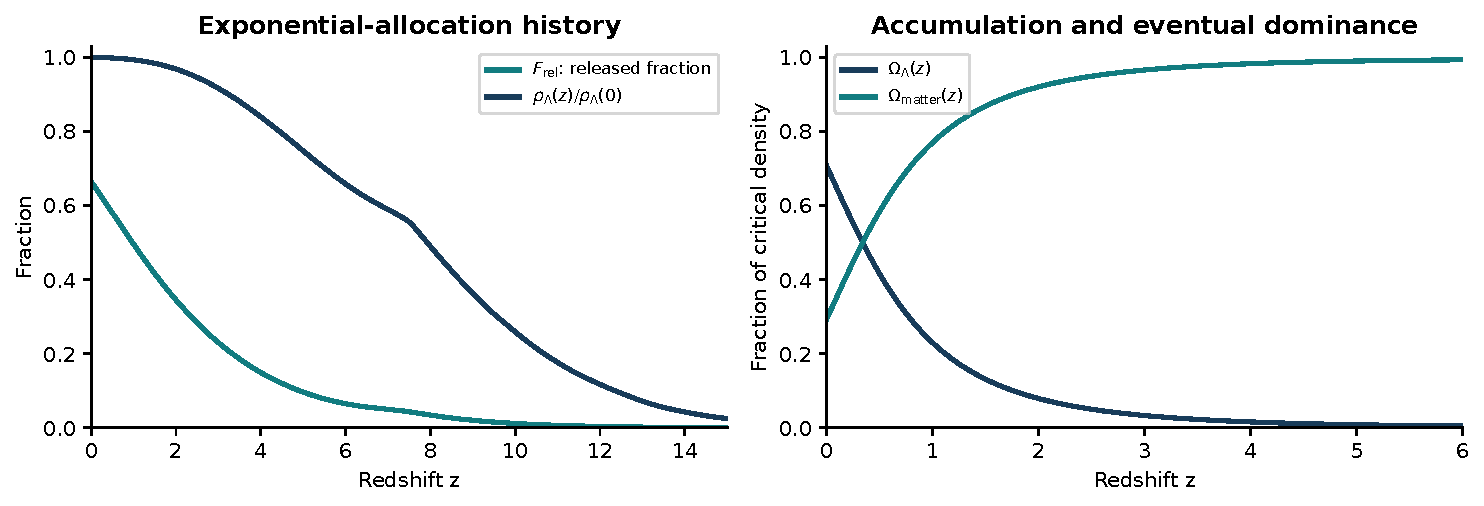
\includegraphics[width=\textwidth]{figures/release_history.pdf}
\caption{The fitted exponential-allocation release history from the
table. The released fraction counts cohorts; the vacuum density weights
their release by the physical matter density at that epoch. The right
panel shows why a substantial early vacuum density becomes dynamically
important only much later. These curves condition on the fitted kernel
and fixed reference assembly history.}
\end{figure}

\subsection{What the hydrodynamic measurement finds}

The archived Gadget-4 calculation measures progenitor information during
self-gravitating assembly. It follows $2\times96^3$ particles in a
$0.75\,h^{-1}$ comoving Mpc box, from initial conditions at $z=63$ to
$z=6$, with 48 analysis snapshots between $z=15$ and 6. Primordial
hydrogen/helium cooling and a star-formation prescription are included.
The cohort consists of the gas particles in a host at first entry.
Progenitor labels come from group membership one dynamical time earlier;
ungrouped gas is divided into spatial octants. Several partitions of
the current host measure the remaining label information. \source{C2}

Approximately half of the resolved label information is already lost at
entry. The measured kernels are fitted by
\begin{equation}
K_{\rm mix}(\tau)=1-(1-K_0)e^{-\tau/\tau_{\rm mix}},
\qquad K_0\simeq0.5.
\end{equation}
The subsequent decay takes a few dynamical times. Because this kernel
includes an immediate component, its fitted tail time cannot be directly
equated with the pure-exponential $f$ in the cosmological fit. The
appropriate comparison convolves each measured kernel with its
corresponding first-entry history.

\begin{table}[htbp]
\centering\small
\begin{tabular}{lrrr}
\toprule
Retention gate & Hosts & $I_{\rm rel}$ across partitions & Reference target \\
\midrule
$17\,\kms$ & 3 & $75.4$--$75.9$ & $94.2$ \\
$14\,\kms$ & 10 & $93.1$--$96.7$ & $94.2$ \\
$12\,\kms$ & 16 & $108.0$--$109.9$ & $94.2$ \\
\bottomrule
\end{tabular}
\caption{The measured mixing histories after convolution with assembly.
Ranges show changes among spatial partitions, not statistical confidence
intervals. Retention gates were imposed in the analysis.}
\end{table}

At the reference $17\,\kms$ gate, the measured integral is about $20\%$
too small. A $14\,\kms$ gate brings it into the required range. That
agreement identifies a physical possibility, but selecting a gate after
examining the integral does not independently predict its normalization.
At the reference gate, changing the lookback time of the labels moves
the integral to $82$--$83$; using only grouped gas moves it to $57$--$65$.
The definition of the retained source record is therefore consequential.

The run resolves only about 500--2400 gas particles per host, includes
three hosts at the reference gate, and omits molecular cooling, feedback,
and explicit subgrid diffusion. Its spatial partitions scale with the
evolving halo radius. A physical prediction requires label and resolution
rules fixed by the theory, gas-retention thresholds measured from the
simulation, and convergence under improved gas resolution and transport
physics. The present run supports a measurable assembly-and-mixing
mechanism while leaving its absolute release rate unsettled.

\begin{figure}[htbp]
\centering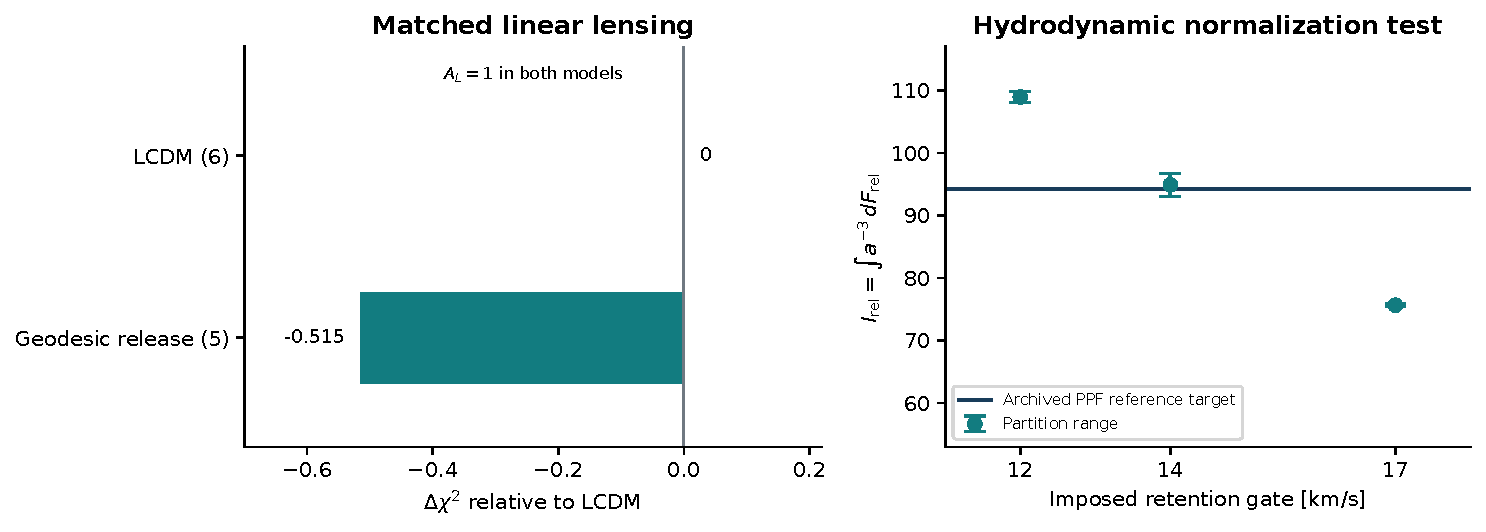
\includegraphics[width=\textwidth]{figures/cosmology.pdf}
\caption{Left: the matched linear-lensing likelihood comparison, with
cosmological parameter counts in parentheses. Right: the archived
hydrodynamic kernels compared with the linear-depletion PPF reference
target $I_{\rm rel}=94.2$. The ranges describe partition choices; the
positive-allocation model uses a different weighted integral.}
\end{figure}

\subsection{The vacuum density from the retention gate}
\label{sec:coolinggate}

Equation~\eqref{eq:flatness} turns the release integral into a vacuum
density. With $\omega_b=0.02238$ and the tied abundance, $I_{\rm rel}$
alone fixes $h$ and $\Omega_\Lambda$. The integral weights each released
cohort by the matter density at its release, $a^{-3}$, so the earliest
retaining halos dominate it. Their number is set by the retention gate,
the threshold above which a halo keeps cooling gas in which progenitor
labels mix. A lower gate admits more halos at earlier times and raises the
integral.

The construction places records in condensed baryons: stars and gas that
has cooled. Shock-heated gas whose cooling time exceeds its dynamical time
carries none. A newly assembled halo therefore enters the release history
when its virialized gas can cool within one dynamical time. This is the
atomic-cooling limit of first-galaxy formation. For primordial gas in
collisional ionization equilibrium, with atomic hydrogen and helium
cooling \cite{katz96}, Compton cooling on the microwave background, and
no molecular hydrogen or ultraviolet background, the condition
$t_{\rm cool}=R_{\rm vir}/V_{\rm vir}$ at the mean virial gas density gives
$T_{\rm gate}=(0.99$--$1.07)\times10^4\,$K for $30\ge z\ge8$. Collisional
excitation of hydrogen sets this temperature. Its rate rises by three
orders of magnitude between $8\times10^3$ and $1.5\times10^4\,$K, so the
threshold barely moves with density or redshift. The virial relation
$T_{\rm vir}=\mu m_pV_{\rm vir}^2/2k_B$ converts it to a circular velocity.
Gas at the threshold is nearly neutral, $\mu=1.22$, which gives
$V_{\rm gate}=11.6$--$12.0\,\kms$. The reference gate of $17\,\kms$ is the
same temperature evaluated for fully ionized gas, $\mu=0.59$.

The archived run measures a condensation threshold. Its group catalogues record
the star-forming gas and stellar mass of every group at each snapshot.
The fraction of groups holding condensed baryons rises from below $0.1$
to unity across $0.03\,$dex in virial velocity and reaches one half at
$8.6$, $8.9$, $9.3$ and $10.2\,\kms$ for $z=11$--15, 9--11, 7.5--9 and
6--7.5. Halo centres are denser than the virial mean, so gas condenses
in smaller halos than the mean-density estimate allows. Using this
threshold as the release gate assumes that condensed baryons identify
recoverable source records.

Table~\ref{tab:coolinggate} recomputes the first-entry history at each
pre-reionization gate and convolves it with the measured kernels. The
post-reionization gate stays at $30\,\kms$ and reionization at
$z_{\rm re}=7.66$. The six kernels measured on the ten hosts at $14\,\kms$
and the sixteen hosts at $12\,\kms$ change $I_{\rm rel}$ by at most $6\%$
at fixed gate, so the gate controls the result. The three hosts at
$17\,\kms$ have a slower tail and give the integral $75.4$--$75.9$ listed
above.

\begin{table}[htbp]
\centering\small
\begin{tabular}{lrrrr}
\toprule
Origin of the pre-reionization gate & $V_{\rm gate}$ ($\kms$) & $I_{\rm rel}$ & $h$ & $\Omega_\Lambda$ \\
\midrule
Run, condensed baryons, $z=9$--15 & 9 & $128.6$--$135.7$ & $0.77$--$0.79$ & $0.766$--$0.775$ \\
Run, condensed baryons, $z=6$--9 & 10 & $118.9$--$125.4$ & $0.75$--$0.77$ & $0.752$--$0.761$ \\
Cooling criterion, neutral gas & 12 & $103.7$--$109.5$ & $0.71$--$0.73$ & $0.725$--$0.736$ \\
Gate selected by the likelihood & 14 & $92.4$--$97.5$ & $0.69$--$0.70$ & $0.702$--$0.713$ \\
Ionized conversion of cooling temperature & 17 & $80.9$--$85.3$ & $0.65$--$0.67$ & $0.673$--$0.685$ \\
\bottomrule
\end{tabular}
\caption{Release integral, Hubble parameter and vacuum fraction from
Equation~\eqref{eq:flatness} against the pre-reionization retention gate.
Ranges span the six kernels measured at the $12$ and $14\,\kms$ gates.
The archived linear-depletion likelihood requires $I_{\rm rel}=94.2\pm0.8$, $h=0.689$ and
$\Omega_\Lambda=0.707$.}
\label{tab:coolinggate}
\end{table}

Both gates computed without feedback lie below the gate that the
likelihood selects. The cooling criterion gives $\Omega_\Lambda=0.73$ and
the run gives $0.75$--$0.77$. Supernova feedback and photoheating inside
ionized regions before the global reionization redshift remove gas from
the smallest halos and raise the effective gate
\cite{thoul96,okamoto08}. The run contains neither process. Gates from
$12$ to $17\,\kms$ span the neutral and ionized conversions of the
cooling temperature. Across that range $\Omega_\Lambda=0.67$--$0.74$, and
the vacuum density lies between $14\%$ below and $16\%$ above the
likelihood value.

The cooling-criterion calculation uses $\eta_*$, the formation abundance,
assembly of the measured fluctuation spectrum, the measured mixing kernel
and the atomic-hydrogen cooling threshold. It gives
$I_{\rm rel}=103.7$--$109.5$, $10$--$16\%$ above the archived target
$94.2$, and $\Omega_\Lambda=0.725$--$0.736$ against $0.707$. Condensation
in the no-feedback run gives $I_{\rm rel}=118.9$--$135.7$. Neither
calculation includes feedback. The likelihood selects a gate of
$14\,\kms$, about $5\times10^7\Msun$ at $z\simeq10$.

A retained well is a halo that keeps gas able to cool, in which
progenitor labels mix. The post-reionization gate measures this retention
for photoheated gas \cite{okamoto08}, and the same criterion holds before
reionization. Stars carry records and are collisionless, so they supply
no label mixing; a halo that forms a few stars and then loses its gas
lies outside the gate. The fraction of halos holding star-forming gas
therefore measures the pre-reionization gate. The Renaissance simulations
follow Population~III and metal-enriched star formation with radiative
transfer, radiative and supernova feedback, metal cooling and
Lyman--Werner backgrounds to $z=15$, $12.5$ and $8$ in rare-peak, normal
and void regions \cite{oshea15,xu16}. About $10\%$ of halos of
$10^7\Msun$ host star formation younger than $20\,$Myr, about half of
those of $10^8\Msun$ do, and all above $10^{8.5}\Msun$ do, nearly
independently of redshift and region. Treating this occupation as the
probability that a trajectory's gate lies below a given mass, and using
the linearity of the release integral in the first-entry history,
Table~\ref{tab:retentiongate} gives the result. No input in the chain is
adjusted to the vacuum density.

\begin{table}[htbp]
\centering\small
\begin{tabular}{lrrr}
\toprule
Pre-reionization gate & $I_{\rm rel}$ & $h$ & $\Omega_\Lambda$ \\
\midrule
Sharp, $10^{7}\Msun$ & $137$--$145$ & $0.81$ & $0.78$ \\
Sharp, $10^{7.5}\Msun$ & $104$--$109$ & $0.72$ & $0.73$ \\
Sharp, $10^{8}\Msun$ & $80$--$84$ & $0.66$ & $0.68$ \\
Renaissance occupation & $92.3$--$97.4$ & $0.693$ & $0.709$ \\
\bottomrule
\end{tabular}
\caption{Release integral, Hubble parameter and vacuum fraction with a
mass gate before reionization. The post-reionization gate is
$30\,\kms$ and $z_{\rm re}=7.66$. Ranges span the six measured kernels.
The likelihood requires $I_{\rm rel}=94.2\pm0.8$, $h=0.689$ and
$\Omega_\Lambda=0.707$.}
\label{tab:retentiongate}
\end{table}

The kernels move the occupation result by $\pm2.5$ in $I_{\rm rel}$, the
shape of the occupation curve by $+4/-2.4$, the reionization redshift
$z_{\rm re}=6.94$--$8.40$ by $\pm5.5$, and a post-reionization gate of
$25$--$35\,\kms$ by $\pm4.3$. In quadrature,
\begin{equation}
I_{\rm rel}=95.5\pm8,\qquad \Omega_\Lambda=0.709^{+0.017}_{-0.019},
\qquad h=0.693\pm0.021,
\end{equation}
against the required $94.2$, $0.707$ and $0.689$. Every term of the
flatness sum is fixed once the baryon density is measured: the tie gives
the committed density $5.333\,\omega_b$, the release gives
$\omega_\Lambda=\eta_*\omega_cI_{\rm rel}$, and flatness gives $h^2$ as their
sum. The boxed $h$ is therefore a prediction,
$H_0=69.3\pm2.1\,\mathrm{km\,s^{-1}\,Mpc^{-1}}$, with no fitted dark-sector
parameter, and $h$ varies nearly as $\omega_b^{1/2}$. The reionization
redshift and the post-reionization gate dominate the error. The Milky Way
satellite census places the half-occupation peak mass for any star
formation near $10^{7.5}\Msun$ \cite{nadler20}; those faint galaxies form
a few thousand solar masses of stars and lose their gas, so they lie
below the retention gate. For comparison, the standard quantum estimate
of the vacuum energy exceeds the measured value by about $10^{120}$, and
\LCDM\ fits $\Omega_\Lambda$ as a free constant. A measured cold-gas
retention fraction at $z\ge8$, a tighter reionization redshift and a
feedback-resolved mixing kernel sharpen the test; a converged integral
that differs from the target by more than its uncertainty falsifies the
normalization.

The occupation gate, the measured kernels and the post-reionization gate
fix the release history once the reionization redshift is given, and the
optical depth measures that redshift. Taking $z_{\rm re}$ from the fitted
$\tau$ removes the mixing time, and the release model has four
cosmological parameters against six for \LCDM. In the matched likelihood
with $\sum m_\nu=0.06\,$eV, nonlinear lensing and free calibration the
frozen history gives $\chi^2=2240.100$ against $2239.031$ for \LCDM,
$\Delta\chi^2=+1.07$, at $z_{\rm re}=8.12$, $\tau=0.0587$, $I_{\rm rel}=92.0$
and $H_0=68.42$. With massless neutrinos, fixed calibration and the
low-redshift offset it gives $2226.483$ against $2226.767$. The extreme
kernels and post-reionization gates of $25$--$35\,\kms$ give
$\Delta\chi^2=+1.1$ to $+2.6$. Holding $z_{\rm re}$ at $7.66$ independently
of $\tau$ gives $\Delta\chi^2=+20.2$ and $+4.0$, so the frozen history
predicts that a larger optical depth accompanies a smaller vacuum density.
With $a_0=\epsilon cH_0$ the first fit gives
$a_0=1.249\times10^{-10}\,\mathrm{m\,s^{-2}}$, and the astrophysical chain
without cosmological data gives $(1.27\pm0.04)\times10^{-10}\,\mathrm{m\,s^{-2}}$,
against $1.20\times10^{-10}\,\mathrm{m\,s^{-2}}$ from rotation curves
\cite{lelli17}. Neither uses galactic data.
\source{C2, C7, C8}

\subsection{Equation of state, vacuum energy, and decisive tests}

The vacuum stress has intrinsic $w_\Lambda=p_\Lambda/\rho_\Lambda=-1$.
Its density grows because it receives energy. If one describes this
growing density by a fictitious separately conserved fluid, its inferred
equation of state is
\begin{equation}
w_{\rm eff}=-1-\frac{1}{3}\frac{d\ln\rho_\Lambda}{d\ln a}
=-1-\frac{Q}{3H\rho_\Lambda}\le-1.
\end{equation}
This effective phantom sign comes from energy transfer. A reconstructed
decrease of the physical vacuum density would contradict the monotone
release law, provided the matter transfer and observational systematics
were modeled consistently. A fitted $w_0,w_a$ curve under conserved-CDM
assumptions is a different inference problem; its crossing of $-1$
cannot alone decide this interacting model.

Normalized microscopic probabilities are unchanged by a common shift
of their energy origin. Coupling to gravity also requires the absolute
stress-energy assigned to that origin. The current cosmological
construction selects zero initial vacuum density and generates the
subsequent density through release. Establishing that selection from the
microscopic gravitational theory remains necessary to claim a solution
of the absolute vacuum-energy problem. The empirical fit tests the
generated component under the selected initial condition.

The saved exponential-allocation calculation evolves the geodesic-clock perturbations with
zero rest-frame sound speed and $A_L=1$. Nonlinear lensing corrections
are disabled in both models, and the late-radiation truncation that
introduced reference-split dependence is disabled. The assembly table
retains its reference power spectrum while cosmological parameters vary.
Both models use massless neutrinos with $N_{\rm eff}=3.044$ and the
same simplified low-$\ell$ treatment. \source{C4, C5}

A full test requires a validated nonlinear response, assembly recomputed
for the sampled cosmology, the full low-$\ell$ likelihood, and an
independently measured release kernel. The selected depletion completion below inherits the cold linear fit;
its nonlinear spatial predictions require a separate test.
The present result demonstrates near-equal fit quality with a
microscopically tied abundance and a physically interpretable release
parameter in the specified pipeline.

\subsection{A self-limiting local completion and its coupling}
The unit-clock action is exact above a selected depletion threshold.
For $X=-\nabla_\mu\phi\nabla^\mu\phi/2$, a covariant continuation is
\begin{equation}
P=\lambda X-e-V,\quad L=3(K-V)>0,\quad
e=\frac\lambda2+\frac{2[L-\lambda]_+^3}{3L^2},\quad \lambda\ge L/2.
\end{equation}
The constant $K$ is a minimum total energy. For $\lambda>L$ the
Lagrangian is exactly $\lambda(X-1/2)-V$. On the intermediate branch
$r=\lambda/L\in(1/2,1)$, define $v=\sqrt{2X}$ and $j=\lambda v$.
Then $X=1/2-2(1-r)^2$ and
\begin{equation}
\dot j=-\left[\theta+\frac{V_\phi A(r)j}{\lambda^2}\right]j,
\qquad A(r)=\frac{1+2r-2r^2}{3-2r}\in[3/4,1].
\end{equation}
For regular flow with $K-V$ bounded away from zero, the current stays
nonnegative. Its depleted homogeneous endpoint has $j=0$,
$\rho=K$, $p=-K$. The regular sound speed lies between zero and one.
The constant minimum removes the scalar force at rest. This slows the
source field relative to proper time; no universal atomic-clock effect
has been established. The cubic and floor are constitutive choices.
\source{D1}

For the fitted history, the choice
$K=V(1)+B[e^{-\eta_*F(1)}-e^{-\eta_*}]$ bounds all remaining future
release under the stated monotonicity assumptions. The saved value is
$K=0.3369964$ in units $3H_{100}^2/(8\pi G)$, with
$\max_{a\le1}L/\bar C=0.0299937$. The background and a neighborhood of
its linear perturbations stay on the original branch. Hence the
completion inherits the fitted cold adiabatic linear cosmology. Deep
voids enter a pressure regime with a changed minimum energy and require
new expansion, profile, and lensing predictions. Nonzero-null-gradient
interfaces and nonlinear caustics remain unresolved.

A finite-work contact extends this mechanism to redistribution. For
a transition $E\to E'$ toward target $h$, let
$Q=\Theta\ln(h'/h)$, $W=E'-E+Q$, $U'=U-W$, and $E_B'=E_B+Q$.
Their total energy is conserved. A symmetric gate $v(U)v(U-W)$ allows
only admissible endpoints and vanishes at the floor. Central pair
impulses give reciprocal momentum exchange. The target and physical
rate require selection beyond detailed balance. \source{D2}

A warm fluid stress stores heat as $e_T=z n^\gamma\ge0$ with
$1<\gamma\le2$ and
$\rho=R_0(n,\phi)+e_T$, $p=p_0+(\gamma-1)e_T$.
Its sound speed is an enthalpy-weighted average of the cold speed squared
and $\gamma-1$, preserving the causal local bound and energy floor.
The gate $g=n\mu/(\lambda_0+\gamma e_T)\in[0,1]$ retains a regular
signed power $gB_c$ and reduces to the cold $v_0^2$ gate.
In the selected $\gamma=4/3$ compression test, five resolutions up to
2048 cells conserve mean total energy to $4.9\times10^{-15}$ and keep
positive current. Generated heat falls from 0.0641 to 0.0140 under
refinement, so physical dissipation has not converged. A separate
particle-feedback test has fractional energy error $1.02\times10^{-5}$
and stops short of the target when available work is insufficient.
These tests establish a conservative effective implementation; the
coupled spatial and multistream evolution remains to be validated.
\source{D2}
